%%%%%%%%%%%%%%%%%%%%%%%%%%%%%%%%%%%%%%%%%%%%%%%%%%%%%%%%%%%%%%%%%%%%%%%%%%%
%% This file is part of the book
%%
%% Algorithmic Graph Theory
%% http://code.google.com/p/graph-theory-algorithms-book/
%%
%% Copyright (C) 2009, 2010 Minh Van Nguyen <nguyenminh2@gmail.com>
%%
%% See the file COPYING for copying conditions.
%%%%%%%%%%%%%%%%%%%%%%%%%%%%%%%%%%%%%%%%%%%%%%%%%%%%%%%%%%%%%%%%%%%%%%%%%%%

%% digraph
\subfigure[]{
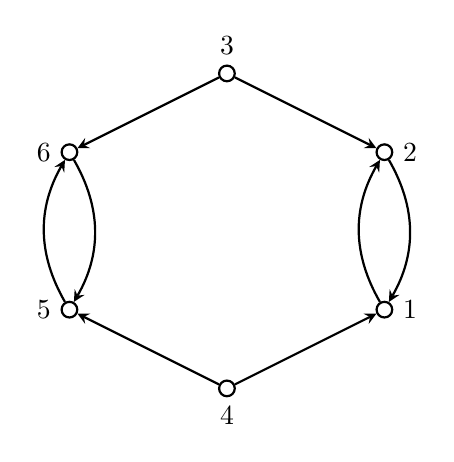
\begin{tikzpicture}
[nodedecorate/.style={shape=circle,inner sep=2pt,draw,thick},%
  arrowdecorate/.style={->,>=stealth,thick},%
  linedecorate/.style={-,thick}]
%% nodes or vertices
\foreach \nodename/\x/\y/\direction/\navigate in {1/2/1/right/east,
  2/2/3/right/east, 3/0/4/above/north, 4/0/0/below/south,
  5/-2/1/left/west, 6/-2/3/left/west}
{
  \node (\nodename) at (\x,\y) [nodedecorate] {};
  \node [\direction] at (\nodename.\navigate) {$\nodename$};
}
%% edges or lines
\path
(1) edge[arrowdecorate,bend left] node {} (2)
(2) edge[arrowdecorate,bend left] node {} (1)
(3) edge[arrowdecorate] node {} (2)
(3) edge[arrowdecorate] node {} (6)
(4) edge[arrowdecorate] node {} (1)
(4) edge[arrowdecorate] node {} (5)
(5) edge[arrowdecorate,bend left] node {} (6)
(6) edge[arrowdecorate,bend left] node {} (5);
\end{tikzpicture}
}
\quad
%%
%% graph
\subfigure[]{
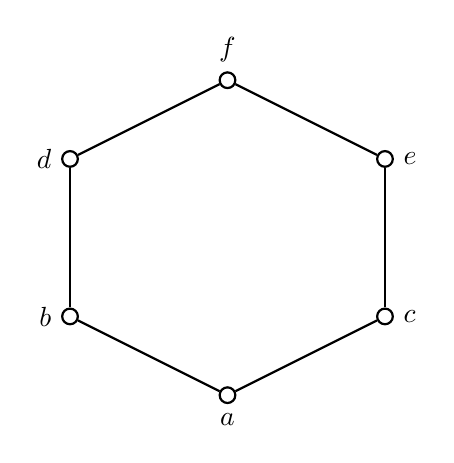
\begin{tikzpicture}
[nodedecorate/.style={shape=circle,inner sep=2pt,draw,thick},%
  linedecorate/.style={-,thick}]
%% nodes or vertices
\foreach \nodename/\x/\y/\direction/\navigate in {c/2/1/right/east,
  e/2/3/right/east, f/0/4/above/north, a/0/0/below/south,
  b/-2/1/left/west, d/-2/3/left/west}
{
  \node (\nodename) at (\x,\y) [nodedecorate] {};
  \node [\direction] at (\nodename.\navigate) {$\nodename$};
}
%% edges or lines
\path
\foreach \startnode/\endnode in {c/e, c/a, e/f, f/d, a/b, b/d} {
  (\startnode) edge[linedecorate] node {} (\endnode)
};
\end{tikzpicture}
}
